\section{Nedunchezhiyan mm20b043}
\subsection{coulomb force}

coulomb force is the force between two stationary electric charge particle.The equation of coulumb force is given by:
\begin{equation}
F=\frac{1}{4\pi \epsilon_0}\frac{q_1 q_2}{r^2}
\label{eqn:coulomb}
\end{equation}
\begin{figure}{h}
 \begin{center}
    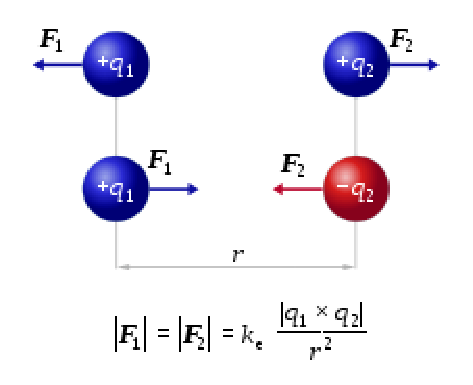
\includegraphics[scale=0.6]{mm20b043.eps}
    \end{center}
\caption{coulomb force between electric charges}
\label{fig:coulomb force}
\end{figure}

\subsubsection{Terms used in the equation}
\begin{itemize}
 \item F-Electrostatic force
 \item$\epsilon$-constant
 \item$\frac{q_1 q_2}{r^2}$-product of magnitude of two charges divided by square of distance between two charges
\end{itemize}

\subsubsection{importance of coulomb force}
coulomb force obtained by using the equation above helps us to find force between two electrically charged particles which is essential in development of theory of electromagnet>\cite{ref1}
\end{document}
